\chapter{Introduction to the DWARF format\label{cha:chapter2}}

To establish correspondence between high-level source code and low-level machine
code, one wants to:
\begin{itemize}
    \item collect all information generated in the compiling process,
    \item and represent that information in a suitable format usable by
        debuggers, concisely and in a compact manner.
\end{itemize}

DWARF is a debugging data format allowing support for source level debugging.

\begin{itemize}
%(linker/assembler)
    \item it is language agnostic, independent of compiler tooling, target architecture and debuggers.
    \item it is somewhat object file agnostic, although it was designed along
        with the ELF object file format.
    \item it is standardized, meaning it has specifications and norms codified into
        a formal document. A commitee oversees extensions to the standard to
        follow the appearance of programming languages and their evolution.
\end{itemize}

\section{Storage}

DWARF data is emitted by the compiler at the code generation step.
At the assembling step, it is stored in particular sections in the object file.
When linking the final binary, the DWARF sections of each object file are
put together in their common corresponding section.

Here is a description of relevant DWARF sections and their contents:

\begin{description}[labelwidth=\widthof{\bfseries .debug\_abbrev},align=parright]
    \item[.debug\_abbrev] -- Abbreviations used to decode the .debug\_info section
    \item[.debug\_frame] -- \Gls{cfi} table
    \item[.debug\_info] -- Core DWARF data section
    \item[.debug\_line] -- Line number information table
    \item[.debug\_loc] -- Location lists for runtime location of variables and parameters
    \item[.debug\_str] -- String table reference in .debug\_info
\end{description}

Multiple techniques are used to reduce the size of the debugging information:

\begin{itemize}
    \item LEB128, a variable length compression algorithm for storage of
        signed and unsigned integers of arbitrary size.
        It is used in DWARF to encode values of various fields (like attributes).
    \item Some of the section tables can become quite large in size.
        In order to save space, those tables are encoded as bytecode instructions
        to be executed by state machines to obtain their fully expanded form.
\end{itemize}

\section{Structure}

\subsection{Debugging information entry}

In DWARF, the base entity manipulated is called an debugging information entry, or DIE.
A DIE is made of a tag specifying what language construct it describes and a list of attributes giving more details concerning that construct.

A DIE tag can designate for example entities such as:
\begin{description}[labelwidth=\widthof{\bfseries DW\_TAG\_formal\_parameter},align=parright]
    \item[DW\_TAG\_subprogram] -- A subroutine/function
    \item[DW\_TAG\_formal\_parameter] -- An argument within function parameters
    \item[DW\_TAG\_lexical\_block] -- Lexical scoping of local variables
    \item[DW\_TAG\_variable] -- A variable
    \item[DW\_TAG\_base\_type] -- Primitive type not defined in terms of other
        types
\end{description}

An attribute is a name/value couple.
The name attribute indicates what the value represents (name, absolute address,
bytecode, offset, string, integer) and what class of values are supported
It is hence possible for attributes values to reference other DIEs and DWARF sections.

\begin{description}[labelwidth=\widthof{\bfseries DW\_AT\_stmt\_list},align=parright]
    \item[DW\_AT\_name] -- Name of the entry
    \item[DW\_AT\_location] -- Bytecode expressing runtime location of a
        variable
    \item[DW\_AT\_type] -- Reference to a type entry
    \item[DW\_AT\_low\_pc] -- Address of the first machine instruction
    \item[DW\_AT\_high\_pc] -- Address or offset of the first location past the last instruction
\end{description}

A DIE can be nested in another parent DIE, and have siblings and children,

\subsection{Compilation unit}

It designates two entities :

\begin{itemize}
    \item an input source file fed to a compiler,
    \item a DIE entry that starts the DWARF data for the source file it represents.
          It can be represented as a tree with an arbitrary number of children.
          It contains general information about the compilation,
          such as the programming language, the compiler flags used or the source
          file name.
\end{itemize}

The .debug\_info section of a binary made with multiple source files would
typically contain a compilation unit entry for each source file used in the
compilation process.

\subsection{Example}

An example \hyperref[lst:tc]{C program}, \hyperref[lst:asm]{assembly} and
\hyperref[lst:dwa]{DWARF output} can be found in the annexes.

\begin{itemize}
    \item  There is a single DWARF compilation unit with two functions and one
        integer base type.
        The function entries contain information about where they are declared in the source, their names, their visibility as symbols (static to the file or not) and address ranges delimiting which instructions constitute them.

    \item  The f function entry contains several variable entries for local, i and j.
Its frame base address is contained in the rbp register,
and runtime location of its arguments and local variables is specified with an
offset relative to that frame base address, e.g the argument x is located at the
address contained in the rbp register minus 4.
There is a offset to the `int` type entry, it is signed and takes 4 bytes.

    \item j is shadowed by another variable of same name in a block, but both variables
have different frame pointer offsets.

\end{itemize}

The program's assembly instructions are interspersed with DWARF .loc directives mapping sets of
instructions to their respective statement location in the source.
The \gls{cfi} directives indicate where the \gls{cfa} is on the stack at all times, even when the code is optimized.

%7.10.10 .cfi_def_cfa_register register
%.cfi_def_cfa_register modifies a rule for computing CFA. From now on register will be used instead of the old one. Offset remains the same.

%7.10.11 .cfi_def_cfa_offset offset
%.cfi_def_cfa_offset modifies a rule for computing CFA. Register remains the same, but offset is new. Note that it is the absolute offset that will be added to a defined register to compute CFA address.

%7.10.13 .cfi_offset register, offset
%Previous value of register is saved at offset offset from CFA.

%usually role of saved ebp in the function prologue.
%.cfi_def_cfa_offset 16
 %: rbp - 8 is return address, rbp - 16 is CFA

%access to base pointer from previous frame without using (e/r)bp, can be omitted
%with optimizations, is optional

\newpage

\section{The ocplib-dwarf library}

In a effort to learn about the DWARF format during the internship, a library
allowing its users to work with DWARF data programmatically in OCaml was
created.

\vspace{5mm}

It reads and prints DWARF data in a human readable format similar to objdump.
Such a library could find a use in implementing a custom debugger fully in
OCaml.\\
The utility can be found on
GitHub\footnote{\url{http://github.com/ocamlpro/typerex-binutils}}.

\begin{figure}
\centering
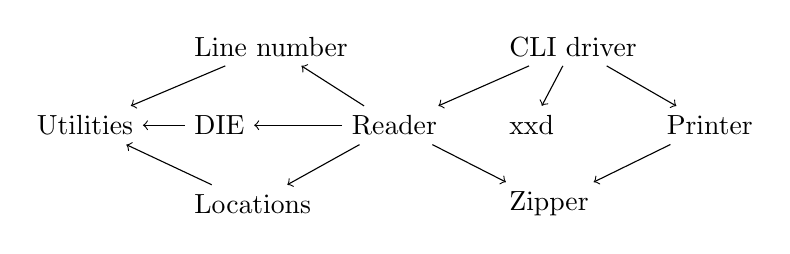
\begin{tikzpicture}[node distance=2cm, anchor=west]

% nodes
\node (A) at (0, 3) {CLI driver};
\node (B) at (2, 2) {Printer};
\node (C) at (-2, 2) {Reader};
\node (D) at (0, 1) {Zipper};

\node (F) at (-4, 3) {Line number};
\node (E) at (-4, 2) {DIE};
\node (G) at (-4, 1) {Locations};
\node (H) at (0, 2) {xxd};
\node (I) at (-6, 2) {Utilities};

\draw [->]
    (A) edge (B) (A) edge (C) (B) edge (D) (C) edge (D)
    (C) edge (E)
    (C) edge (F)
    (C) edge (G)
    (A) edge (H)
    (F) edge (I)
    (E) edge (I)
    (G) edge (I)
    ;
\end{tikzpicture}

\caption{High-level architecture of ocplib-dwarf}
\end{figure}

\begin{itemize}
    \item The driver takes care of the command line option handling.
    \item Each section is parsed in its own module, using utility functions for reading binary data.
        Description of the binary data structure can be found in the DWARF4
        standard\autocite{dwarf4}.
    \item To emulate mutable trees, a zipper library was implemented and used to model
        DIEs, it offers an abstraction that allows DWARF data manipulation.
        If required, the tree can be flattened for serialization and edition of DWARF
        data.
        The DWARF emission writing and editing features are not yet implemented, as
        this task is usually handled by compilers.
    \item One can visualize the DIE tree structure in .debug\_info by outputing it in DOT
        format, then using graphviz to render the graph in an image format.
    \item An hexadecimal view of sections is available for debugging purposes.
        % not used in ocp-lldb, since LLDB already handles that information
        % except for the ptrace primitives, would use FFI
\end{itemize}







